\chapter{Introduction}\label{intro}
The frequency of data access at the users' end has been increased by a large number for the past few years. To ensure low latency at the users' end, it is preferable to reside the data as close to the users as possible. Moreover, in present world data privacy has been a great concern and almost all the nations require the data of their citizens not to reside in some place across their national border. Now its a big concern to maintain privacy regulations and keep foreign countries from being able to subpoena data. To mitigate these two issues, almost all the companies have been building their data centers all around the world. As a result, the sparsity of data has been increased by a huge amount during the last few years.

On the other hand, the amount of data generating in present world is quite large. This huge volume has introduced  a new term ``Big Data". In general ``Big Data" is nothing but the large volume of data that can be both structured and unstructured. The excessive use of social media, scientific instruments, portable devices, sensors are the main reason behind the generation of big data. Data analysis, capture, curation, search, share, storage, transfer, visualization, query, updating, information privacy everything associated with big data has been the challenges of the present world. In case of big data the can be both wide and tall that means the dimension of the data can be quite large. As a result available techniques might not be able to perform the data analysis with the provided limited hardware. Therefore, we need  approaches that have the property of scalability.

For researchers, however, big data brings new sets of challenges like how to efficiently and effectively handle big data in commodity computers, how to apply conventional
algorithms, how
to properly manage big data in distributed setting etc. Specially, in field of
Machine Leaning and
Pattern Recognition, big data poses a threat, because the conventional algorithms
were designed
solely to fulfil its purpose where entire dataset can fit in memory. Distributed
setting was not
taken into consideration. In a nutshell, to extract any meaningful insight from this
big data, we
need powerful tools to analyse it, elastic frameworks to cope up with its sheer
volume and most
importantly we have to rethink and redesign existing algorithms which are most
suitable for
smaller sized dataset and do not take advantage of clusters.


\section{Data Analysis Approaches }
Under these circumstances, we can see that in case of extracting some information from the existing data, we may have to cover a good number of data centres located at different geographical area. This has given the introduction of a new data analysis approach, ``Distributed Data Analysis''. Therefore we get the idea of two approaches of data analysis.

\subsection{Centralized Approach}
The centralized approach to data analysis from distributed data centers is to centralize them first. As shown in Figure \ref{centralized}, this involves a two different steps: 


\begin{enumerate}

\item \textbf{Centralizing step} Data from various data centers are copied into a single data center. It involves recreation of data of all data centers in one location.

\item \textbf{Analysis Step} Process of extracting the necessary information from the centralized data takes place in that single data center. Here traditional intra data center technology is sufficient for the analysis purpose.

\end{enumerate}

\begin{figure}[!htbp]
  \centering
	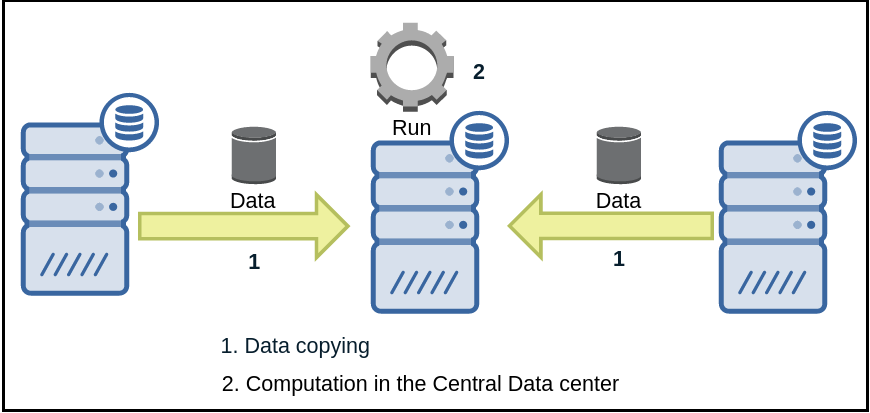
\includegraphics[width=3.2in]{figures/1.png}
	\caption{Centralized Approach}
	\label{centralized}
\end{figure}


This centralized approach is predominant in most practical settings. 
There are mainly two reasons behind its popularity. 
\begin{enumerate}
\item There are lots of frameworks that have already been established for centralized learning approach. That is why centralizing the data is the easiest way to reuse existing data analysis frameworks \cite{1,2,3}
\item Learning algorithms are highly communication intensive. Thus it is assumed that they will note be properly responsive to cross data center execution.
\end{enumerate}
For these reasons, this centralized approach is consistent with reports on the infrastructures of other large organizations, such as Facebook \cite{4}, Twitter \cite{5}, and LinkedIn \cite{6}. 

However the centralized approach has two shortcomings.
\begin{enumerate}
\item While making multiple copy of data at the central data center, it consumes a good amounts of inter data center bandwidth. Since inter data center bandwidth is expensive, it is not easy to increase it according to the necessity \cite{7,8,9,10}.
\item While creating copy of data, it may be a case that data is crossing national borders. However, in current workd data sovereignty is a growing concern that might create a big limitation in this aspect \cite{11,12}.

\end{enumerate}

\subsection{Distributed Approach}
In the distributed approach, raw data is kept in their corresponding data centers. Every data center does a portion of the execution that is only on the data of that data center. The final analysis takes pales by passing small amount of information among the data centers. 

\begin{figure}[!htbp]
  \centering
	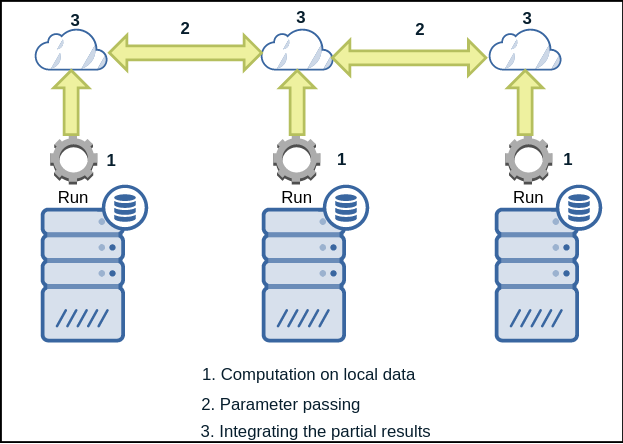
\includegraphics[width=3.2in]{figures/2.png}
	\caption{Distributed Approach}
\label{distributed}
\end{figure}

So according to Figure \ref{distributed}, we can see this approach includes three steps:

\begin{enumerate}
\item \textbf{Local Computation} Whenever the command of starting of any learning process is issued every data center start a partial computation on its own data. They create necessary high level information on data that will be needed in the final computation.

\item \textbf{Parameter Passing} Data centers communicate among themselves and share valuable information.

\item \textbf{Final Computation} By integrating the partial results data centers make the final computational model.
\end{enumerate}

In this way distributed solutions can achieve much lower cross data centers bandwidth utilization, and thus substantially lower cost for large-scale analysis tasks. As the current world has got a concern about `Big Data' and `Data Sovereignty', the distributed approach seems to be more efficient. 


\endinput